\chapter{x86 / x64 architecture}

\section{Data types and representation}
\subsection{Data Types}

\subsubsection{Bits, bytes, words, double words\ldots}
The x86 architecture supports many types of data sizes, which can be used with
various instructions. The following are the most common data types we will be
using with instructions:
\begin{itemize}
    \item byte 	(8 bits) 	\verb+0xab+
    \item word 	(2 bytes) 	\verb+0xabcd+
    \item double word (dword) 	(4 bytes) 	\verb+0xabcdef12+
    \item quad word (qword) (8 bytes) 	(\verb+0xabcdef1234567890+)
    \item double qwords (16 byts)
\end{itemize}

Whenever we use a variable with a certain data type or use a data type with an
instruction, both operands should be of the same size.

\subsubsection{Endianness}

During load and save operations in registers and memories, the bytes are read
in a different order. This byte order is called endianness. Endianness is
distinguished between the little-endian format and the big-endian format.

Big-endian and little-endian are about the order of valence:
\begin{itemize}
    \item In big-endian, the digits with the highest valence are initially. 
    \item In little-endian, the digits with the lowest valence are at the beginning. 
\end{itemize}

Mainframe processors use the big-endian format, some RISC architectures, minicomputers, and in TCP/IP networks, the byte order is also in big-endian format.

Now, let us look at an example with the following values:

\begin{itemize}
        \item Address: \verb+0xffff0000+
        \item Word: \verb+\xAA\xBB\xCC\xDD+
\end{itemize}

\begin{verbatim}
Memory Address 	0xffff0000 	0xffff0001 	0xffff0002 	0xffff0003
Big-Endian 	        AA 	        BB 	        CC 	        DD
Little-Endian 	    DD 	        CC 	        BB 	        AA
\end{verbatim}

\subsubsection{negative number encoding}

\section{Addressing modes}

x86 64-bit processors have 64-bit wide addresses that range from \verb+0x0+ to
\verb+0xffffffffffffffff+, so we expect the addresses to be in this range.
However, RAM is segmented into various regions, like the Stack, the heap, and
other program and kernel-specific regions. Each memory region has specific
read, write, execute permissions that specify whether we can read from it,
write to it, or call an address in it.

Whenever an instruction goes through the Instruction Cycle to be executed, the
first step is to fetch the instruction from the address it's located at. There
are several types of address fetching (i.e., addressing modes) in the x86
architecture.

The addressing modes are the supported methods for accessing a value in memory using
the address of a data item being accessed (read or written). This might include the name
of a variable or the location in an array.

The basic addressing modes are:
\begin{itemize}
    \item Register
    \item Immediate
    \item Memory
\end{itemize}

Each of these modes is described with examples in the following sections. Additionally,
a simple example for accessing an array is presented.

\subsection{Addresses and Values}
On a 64-bit architecture, addresses require 64-bits.
the only way to access memory is with the brackets
(\verb+[]+). Omitting the brackets will not access memory and instead obtain the address of
the item.
\begin{verbatim}
mov rax, qword [var1] ; value of var1 in rax
mov rax, var1 ; address of var1 in rax
\end{verbatim}

When accessing memory, in many cases the operand size is clear.

However, for some instructions the size can be ambiguous. For example,
\begin{verbatim}
inc [rbx] ; error
\end{verbatim}

is ambiguous since it is not clear if the memory being accessed is a byte, word, or
double-word. In such a case, operand size must be specified with either the byte, word,
or dword, qword size qualifier. For example,
\begin{verbatim}
      inc byte [rbx]
      inc word [rbx]
      inc dword [rbx]
\end{verbatim}
each instruction requires the size specification in order to be clear and legal.



\subsection{Register Mode Addressing}
Register mode addressing means that the operand is a CPU register. For
example:
\begin{verbatim}
mov eax, ebx
\end{verbatim}
Both \verb+eax+ and \verb+ebx+ are in register mode addressing.


\subsection{Immediate Mode Addressing}

Immediate mode addressing means that the operand is an immediate value. For
example:
\begin{verbatim}
mov eax, 123
\end{verbatim}
The destination operand, \verb+eax+ , is register mode addressing. The
\verb+123+ is immediate mode addressing. It should be clear that the
destination operand in this example cannot be immediate mode.


\subsection{Memory mode addressing}
Memory mode addressing means that the operand is a location in memory (accessed
via an address). This is referred to as {\bf indirection} or {\bf
dereferencing}

\begin{verbatim}
         mov rax, qword [qNum]
\end{verbatim}

Will access the memory location of the variable \verb+qNum+ and retrieve the value stored
there. This requires that the CPU wait until the value is retrieved before completing the
operation and thus might take slightly longer to complete than a similar operation using
an immediate value.

When accessing arrays, a more generalized method is required. Specifically, an address
can be placed in a register and indirection performed using the register (instead of the
variable name).  For example, assuming the following declaration:
\begin{verbatim}
lst dd 101, 103, 105, 107
\end{verbatim}

The first element of the array could be accessed as follows:
\begin{verbatim}
mov eax, dword [lst]
\end{verbatim}
Another way to access the first element is as follows:
\begin{verbatim}
mov rbx, list
mov eax, dword [rbx]
\end{verbatim}

There are several ways to access the array elements. One is to use a base address and
add a displacement. For example, given the initializations:
\begin{verbatim}
mov rbx, lst
mov rsi, 8
\end{verbatim}


Each of the following instructions access the third element .
\begin{verbatim}
mov eax, dword [lst+8]
mov eax, dword [rbx+8]
mov eax, dword [rbx+rsi]
\end{verbatim}

The general format of memory addressing is as follows:
\begin{verbatim}
[ baseAddr + (indexReg * scaleValue ) + displacement ]
\end{verbatim}
Where \verb+baseAddr+ is a register or a variable name. The \verb+indexReg+ must be a register. The
\verb+scaleValue+ is an immediate value of 1, 2, 4, 8 (1 is legal, but not useful). The
\verb+displacement+ must be an immediate value. 

\section{Registers}

There are many registers in the x86 architecture, but we will only focus on the
ones necessary for learning basic Assembly and essential for future binary
exploitation.

\subsection{Intel 32 bites registers}


\subsubsection{General purpose registers}
\begin{itemize}
    \item \verb+EAX+ Extended Accumulator Register
    \item \verb+EBX+ Extended Base Register
    \item \verb+ECD+ Extended Counter Register
    \item \verb+EDX+ Extended Data Register
    \item \verb+ESI+ Extended Source Index
    \item \verb+EDI+ Extended Destination Index
    \item \verb+EBP+ Extended Base Pointer
    \item \verb+ESP+ Extended Stack Pointer
\end{itemize}

All the general purpose registers are 32-bit size in Intel’s IA-32 architecture but depending
on their origin and intended purpose, a subset of some of them can be referenced in
assembly.
\begin{verbatim}
32 bits         16 bits         8 bits
EAX             AX              AH / AL
EBX             BX              BH / BL
ECX             CX              CH / CL
EDX             DX              DH / DL
ESI             SI
EDI             DI
EBP             BP
ESP             SP
\end{verbatim}

\verb+AX+ to \verb+SP+ are the 16 bit registers used to reference the 16 least
significant bits in their equivalent 32 bit registers. The eight bit registers
reference the higher and lower eight bits of the 16 bit registers.

\subsubsection{Segment registers}
are used to make segmental distinctions in the binary. We will
approach segments later but in short, the hexadecimal value \verb+0x90+ can
either represent an instruction or a data value. The CPU knows which one thanks
to segment registe.

\subsubsection{Status flag registers}
Flags are tiny bit values that are either set (1)
or not set (0). Each flag represent a status. For example, if the “signed” flag
is set, the value of FF will represent a \verb+-1+ in decimal notation instead
of \verb+255+. Flags are all stored in special flag register, were many one bit
flags are stored at once. The flags are set whenever an operation resulted in
certain state or output. The flags we are most interested in for now are:
\begin{itemize}
        \item Z – zero flag, set when the result of the last operation is zero
            32 bits 16 bits 8 bit
        \item S – signed flag, set to determine if values should be intercepted
            as signed or unsigned
        \item O – overflow flag, set when the result of the last operation
            switches the most significant bit from either F to 0 or 0 to F.
        \item C – carry flag, set when the result of the last operation changes
            the most significant bit
\end{itemize}

{\bf Extended Instruction Pointer (EIP)} The instruction pointer has the same
function in a CPU as the needle had in those old gramophones your grandpa used
to have. It points to the next instruction to be executed.


\subsection{Intel 64 bites registers}


\subsubsection{General purpose registers} 

Sixteen general purpose 64-bit registers:
\begin{itemize}
        \item eight  RAX, RBX, RCX, RDX, RBP, RSI, RDI, and RSP. 
        \item eight are named R8-R15.
\end{itemize}

By replacing the initial \verb+R+ with an \verb+E+ on the first eight
registers, it is possible to access the lower 32 bits (\verb+EAX+ for
\verb+RAX+). 

Similarly, for \verb+RAX+, access to the lower 16 bits is possible by removing
the initial \verb+R+ , and the lower byte of the these by switching the
\verb+X+ for \verb+L+ (\verb+AL+ for \verb+AX+), and the higher byte of the low
16 bits using an \verb+H+ (\verb+AH+ for \verb+AX+). 

The new registers \verb+R8+ to \verb+R15+ can be accessed in a similar manner
like this: \verb+R8+ (qword), \verb+R8D+ (lower dword), \verb+R8W+ (lowest
word), \verb+R8B+ (lowest byte MASM style, Intel style \verb+R8L+). Note there
is no \verb+R8H+


 \begin{figure}
  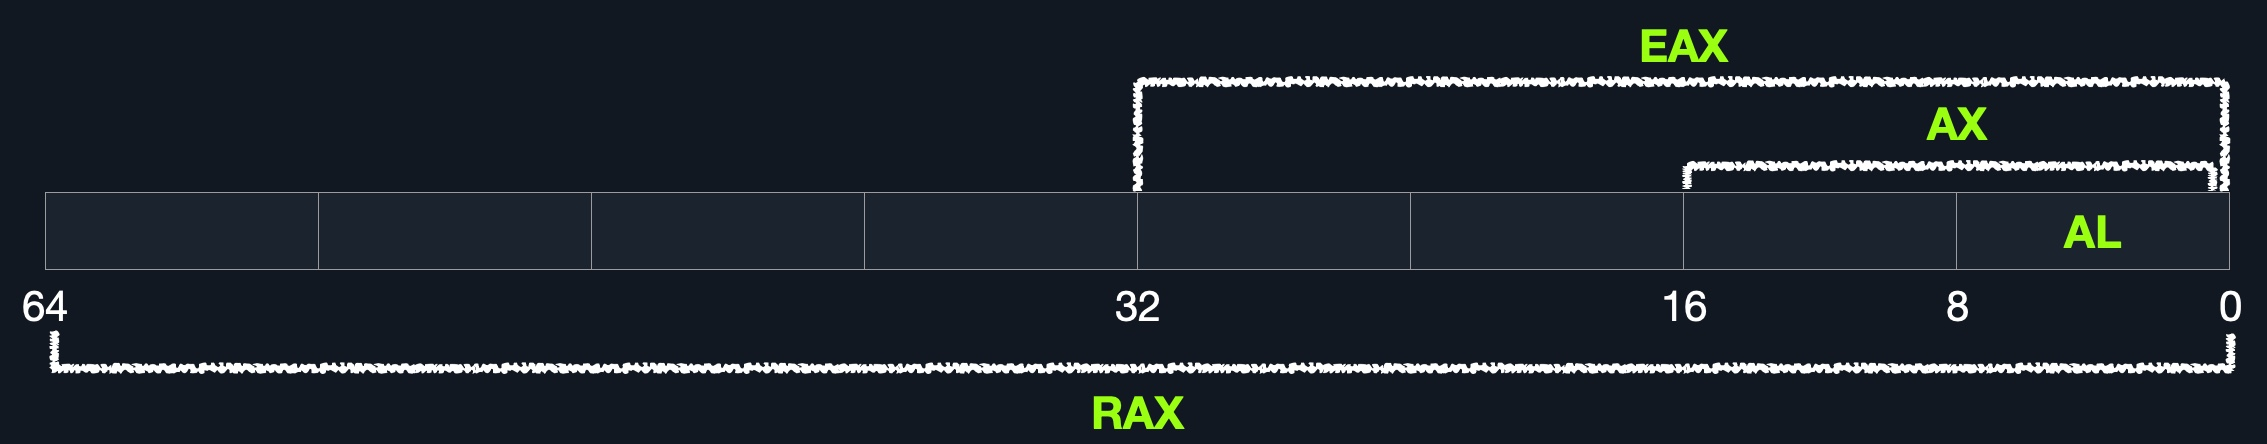
\includegraphics[width=\linewidth]{binary/archi/images/assembly_register_parts.jpg}
  \caption{Registry parts}
  \label{fig:assembly_register_parts}
\end{figure}

\begin{verbatim}
Data/Arguments Registers
    Syscall Number/Return value 	rax 
    Callee Saved 	                rbx 	
    1st arg - Destination operand 	rdi 	
    2nd arg - Source operand  	    rsi 	
    3rd arg 	                    rdx 	
    4th arg - Loop counter 	        rcx 	
    5th arg 	                    r8 	
    6th arg 	                    r9
Pointer Registers
    Base Stack Pointer 	            rbp
    Current/Top Stack Pointer 	    rsp 
    Instruction Pointer 'call only' rip
\end{verbatim}


\section{Instruction set}

Intel instructions vary in size from one to fourteen bytes. The opcode (short
for operation code) is mandatory for them all and can be combined with other
optional or mandatory bytes to create advanced instructions.

\href{http://ref.x86asm.net/coder32.html}{list of all opcodes}


Most instructions have two operators (like \verb+add eax, ebx+), but some have
one (\verb+not eax+) or even three (\verb+imul eax, edx, 64+). Instructions
that contain something with \verb+dword ptr [eax]+ reference the double word
value at memory offset \verb+[XXX]+. Note that the bytes are saved in reverse
order in the memory as Intel uses Little Endian representation. 


\subsection{Arithmetic operations}
\subsubsection{INC / DEC}

\begin{verbatim}
inc dest
dec dest
\end{verbatim}

\subsubsection{ADD / SUB}

\begin{verbatim}
add dest, src
sub dest, src
\end{verbatim}

Destination and source can be either a register,  a memory reference
(\verb+[esp]+)

The source can also be an immediate number.

\subsubsection{DIV / IDIV}

\verb+IDIV+ is the same as \verb+DIV+ but signed division.

\begin{verbatim}
div    divisor
idiv   divisor
\end{verbatim}

The dividend is always \verb+eax+ and that is also were the result of the
operation is stored. The rest value is stored in \verb+edx+.

\begin{verbatim}
mov eax, 65
mov ecx, 4
div ecx
\end{verbatim}

\subsubsection{MUL / IMUL}

\begin{verbatim}
mul value                ; *  eax by value
mul dest, value, value   
mul dest, value
\end{verbatim}

\subsection{Bitwise operations}

\begin{verbatim}
add dest, src
or dest, src
xor dest, src
not eax
\end{verbatim}

\subsection{Data moving}
\subsubsection{mov}
\begin{verbatim}
mov dest, src
movzx dest, src
movzx dest, src
\end{verbatim}

MOV moves data from source into destination. Both source and destination can be
register, or one of them register and the other one a memory reference. Both
cannot be a memory reference however.

The mov instructions come in many flavours, \verb+MOVS/MOVSB/MOVSW/MOVSD+ for
example copy a byte, word or dword from source to destination.

\begin{verbatim}
 +------------------+                  +------------+
 | Registers        |                  | Memory     |
 +------------------+                  +------------+
 | EAX = 0x00000000 |       0x00403A40 | 0x7C81776F |
 | EBX = 0x00403A40 |       0x00403A44 | 0x7C911000 |
 +------------------+       0x00403A48 | 0x0012C140 |
                            0x00403A4C | 0x7FFDB000 |
                                       +------------+
mov eax, [ebx+8]
# eax = 0x0012C140
\end{verbatim}

\subsubsection{lea}

Another instruction that can be used for data moving is the \verb+LEA+
instruction which  stands for “Load Effective Address” and the syntax looks like this:
\begin{verbatim}
lea eax, dword ptr[ecx+edx] ; This will store ecx+edx in eax
\end{verbatim}

\verb+lea+ loads a pointer to the specified value.


\begin{verbatim}
 +------------------+                  +------------+
 | Registers        |                  | Memory     |
 +------------------+                  +------------+
 | EAX = 0x00000000 |       0x00403A40 | 0x7C81776F |
 | EBX = 0x00403A40 |       0x00403A44 | 0x7C911000 |
 +------------------+       0x00403A48 | 0x0012C140 |
                            0x00403A4C | 0x7FFDB000 |
                                       +------------+
lea eax, [ebx+8]
# eax = 0x00403A48
\end{verbatim}

\subsubsection{xchg}

Swap data between two registers or addresses 	
\begin{verbatim}
xchg rax, rbx 
\end{verbatim}

\subsection{Contol instructions}
Program control refers to basic programming structures such as IF statements and
looping.


\subsubsection{Label}
A program label is the target, or a location to jump to, for control statements.
For example: 
\begin{verbatim}
loopStart:
last:
\end{verbatim}


\subsubsection{Unconditional control instruction}
The unconditional instruction provides an unconditional jump to a specific location in
the program denoted with a program label.

\begin{verbatim}
jmp address
\end{verbatim}


\subsubsection{Conditional control instruction}
The conditional control instructions provide a conditional jump based on a comparison.
This provides the functionality of a basic IF statement.

\begin{verbatim}
je  address
jle address
jz  address
...
\end{verbatim}

\begin{verbatim}
jz  	D = 0 	Destination equal to Zero
jnz 	D != 0 	Destination Not equal to Zero
js 	    D < 0 	Destination is Negative
jns 	D >= 0 	Destination is Not Negative (i.e. 0 or positive)
jg 	    D > S 	Destination Greater than Source
jge 	D >= S 	Destination Greater than or Equal Source
jl 	    D < S 	Destination Less than Source
jle 	D <= S 	Destination Less than or Equal Source
\end{verbatim}

Most instructions set one or more flags. Let’s revisit some of the instructions
we already looked at and see which flags they set:
\begin{itemize}
    \item \verb+ADD/SUB+ can set all of the Z, S, O, C flags (and some more
            that are of no interest to us right now) according to the result. 
    \item \verb+AND+ instruction however always clears the O and C flags, but
        sets Z and S flags according to the result.
\end{itemize}

Depending on which flags are set, a jump will either happen or not.

\subsubsection{cmp}

most of the time you will see an instruction \verb+CMP+ being used before a
jump. \verb+CMP+ is the ideal pre-branch instruction as it can set all the
status flags and is really fast. The syntax for \verb+CMP+ is: 
\begin{verbatim}
cmp dest, src
cmp rbx, 10
cmp rbx, rax
\end{verbatim}

This does not mean the other instructions cannot be used
before a jump, for example \verb+XOR+ occurs frequently but the most common is
the \verb+CMP+ instruction.

\subsubsection{Jump Out of Range}
The target label is referred to as a short-jump. Specifically, that means the target label
must be within 128 bytes from the conditional jump instruction. While this limit is
not typically a problem, for very large loops, the assembler may generate an error
referring to “jump out-of-range”. The unconditional jump is not limited in range.
If a “jump out-of-range” is generated, it can be eliminated by reversing the logic and
using an unconditional jump for the long jump.


\subsubsection{Loop}
The \verb+loop+ instruction decrements \verb+ECX+ and jumps to the address
specified by \verb+arg+ unless decrementing \verb+ECX+ caused its value to
become zero. For example: 
\begin{verbatim}
mov ecx, 5
start_loop:
; the code here would be executed 5 times
loop start_loop
\end{verbatim}


\subsection{Stack management}

We will primarily be pushing data from registers into the stack before we call
a function or call a syscall, and then restore them after the function and the
syscall. This is because functions and syscalls usually use the registers for
their processing, and so if the values stored in the registers will get changed
after a function call or a syscall, we will lose them.

\subsubsection{push}
PUSH decrements the stack pointer (\verb+ESP+) to point to the new
top of the stack.
\begin{verbatim}
push var/reg
\end{verbatim}

\subsubsection{pop}
POP  increments the stack pointer (\verb+ESP+) to point to the new
top of the stack.
\begin{verbatim}
pop dest
\end{verbatim}



\subsection{Syscall}

\subsubsection{Syscalls (linux)}
SYSCALL invokes an OS system-call handler at privilege level 0.

A syscall takes the required arguments in the registers and executes the
function with the provided arguments. 

{\bf Syscall Function Arguments}: 

To find the arguments accepted by a syscall, we can use the \verb+man -s 2+
command with the syscall name.

{\bf Syscall Calling Convention}: 

To call a syscall, we have to:
\begin{enumerate}
    \item    Save registers to stack
    \item    Set its syscall number in rax
    \item    Set its arguments in the registers
    \item    Use the syscall assembly instruction to call it
\end{enumerate}

{\bf Syscall Arguments}: 

\begin{verbatim}
Description 	                64-bit Register 	8-bit Register
Syscall Number/Return value 	rax             	al
Callee Saved 	                rbx             	bl
1st arg 	                    rdi             	dil
2nd arg 	                    rsi             	sil
3rd arg 	                    rdx             	cl
4th arg 	                    rcx             	bpl
5th arg 	                    r8 	                r8b
6th arg 	                    r9 	                r9b
\end{verbatim}
Any additional arguments can be stored in the stack (though not many syscalls
use more than 6 arguments.).


\subsection{Functions}

function call rely heavily on convention that are described
\href{https://en.wikipedia.org/wiki/X86_calling_conventions}{here}

\subsubsection{Declaration}

A function must be written before it can be used.  Functions are located in the
code segment. The general format is:
\begin{verbatim}
    global <procName>
    <procName>:
      ; function bodY
    ret
\end{verbatim}

\subsubsection{Linkage}
The linkage is about getting to and returning from a function call correctly.
There are two instructions that handle the linkage, \verb+call <funcName>+ and
\verb+ret+ instructions.

The \verb+call+ transfers control to the named function, and \verb+ret+ returns
control back to the calling routine.
\begin{itemize}
    \item The call works by saving the address of where to return to when the
        function completes (referred to as the return address). This is
        accomplished by placing contents of the \verb+rip+ register on the
        stack. Recall that the rip register points to the next instruction to
        be executed (which is the instruction immediately after the call).

    \item  The ret instruction is used in a procedure to return. The ret
        instruction pops the current top of the stack (\verb+rsp+) into the
        \verb+rip+ register. Thus, the appropriate return address is restored.
\end{itemize}

Since the stack is used to support the linkage, it is important that within the
function the stack must not be corrupted. Specifically, any items pushed must
be popped. Pushing a value and not popping would result in that value being
popped off the stack and placed in the rip register. This would cause the
processor to attempt to execute code at that location. Most likely the invalid
location will cause the process to crash.


\subsubsection{Argument Transmission}
Argument transmission refers to sending information (variables, etc.) to a
function and obtaining a result as appropriate for the specific function.

The standard terminology for transmitting values to a function is referred to
as call-by- value. The standard terminology for transmitting addresses to a
function is referred to as call-by-reference. This should be a familiar topic
from a high-level language.

\subsubsection{x86 C calling Convention (cdecl)}

\begin{itemize}
    \item {\bf The Caller’s Rules}: The caller should adhere to the following
        rules when invoking a subroutine:
        \begin{itemize}
            \item Before calling a subroutine, the caller should save the
                contents of certain registers that are designated caller-saved.
                The caller-saved registers are \verb+EBX+, \verb+ECX+,
                \verb+EDX+. If you want the contents of these registers to be
                preserved across the subroutine call, push them onto the
                stack.
            \item To pass parameters to the subroutine, push them onto the
                stack before the call. The parameters should be pushed in
                inverted order (i.e. last parameter first) since the stack
                grows down, the first parameter will be stored at the lowest
                address (this inversion of parameters was historically used to
                allow functions to be passed a variable number of parameters).
            \item To call the subroutine, use the call instruction. This
                instruction places the return address on top of the parameters
                on the stack, and branches to the subroutine code.
            \item After the subroutine returns, (i.e. immediately following the
                call instruction) the caller must remove the parameters from
                stack. This restores the stack to its state before the call was
                performed.
            \item The caller can expect to find the return value of the
                subroutine in the register \verb+EAX+.  
            \item The caller restores the contents of caller-saved registers
                (\verb+EBX+, \verb+ECX+, \verb+EDX+) by popping them off of the
                stack. The caller can assume that no other registers were
                modified by the subroutine.
        \end{itemize}
    \item {\bf The Callee’s Rules}: The definition of the subroutine should
        adhere to the following rules:
        \begin{itemize}
            \item At the beginning of the subroutine, the function should push
                the value of \verb+EBP+ onto the stack, and then copy the value
                of \verb+ESP+ into \verb+EBP+ using the following instructions:
\begin{verbatim}
        push ebp
        mov ebp, esp
\end{verbatim}
                The reason for this initial action is the maintenance of the
                base pointer, \verb+EBP+. The base pointer is used by
                convention as a point of reference for finding parameters and
                local variables on the stack. Essentially, when any subroutine
                is executing, the base pointer is a “snapshot” of the stack
                pointer value from when the subroutine started executing.
                Parameters and local variables will always be located at known,
                constant offsets away from the base pointer value. We push the
                old base pointer value at the beginning of the subroutine so
                that we can later restore the appropriate base pointer value
                for the caller when the subroutine returns. Remember, the
                caller isn’t expecting the subroutine to change the value of
                the base pointer. We then move the stack pointer into
                \verb+EBP+ to obtain our point of reference for accessing
                parameters and local variables.
            \item Next, allocate local variables by making space on the stack.
                Recall, the stack grows down, so to make space on the top of
                the stack, the stack pointer should be decremented. The amount
                by which the stack pointer is decremented depends on the number
                of local variables needed. For example, if 3 local integers (4
                bytes each) were required, the stack pointer would need to be
                decremented by 12 to make space for these local variables
                (\verb+sub esp, 12+) As with parameters, local variables will
                be located at known offsets from the base pointer.
            \item Next, the values of any registers that are designated
                callee-saved that will be used by the function must be saved.
                To save registers, push them onto the stack. The callee-saved
                registers are \verb+EDI+ and \verb+ESI+.
            \item When the function is done, the return value for the function
                should be placed in \verb+EAX+ if it is not already there.
            \item  The function must restore the old values of any callee-saved
                registers (\verb+EDI+ and \verb+ESI+) that were modified. 
            \item Next, we deallocate local variables. In practice, move the
                value in the base pointer into the stack pointer (i.e.
                \verb+mov esp, ebp+). This trick works because the base pointer
                always contains the value that the stack pointer contained
                immediately prior to the allocation of the local variables.
            \item Immediately before returning, we must restore the caller’s
                base pointer value by popping \verb+EBP+ off the stack.
                Remember, the first thing we did on entry to the subroutine was
                to push the base pointer to save its old value.
            \item Finally, we return to the caller by executing a ret
                instruction. This instruction will find and remove the
                appropriate return address from the stack.
        \end{itemize}
\end{itemize}


 \begin{figure}
  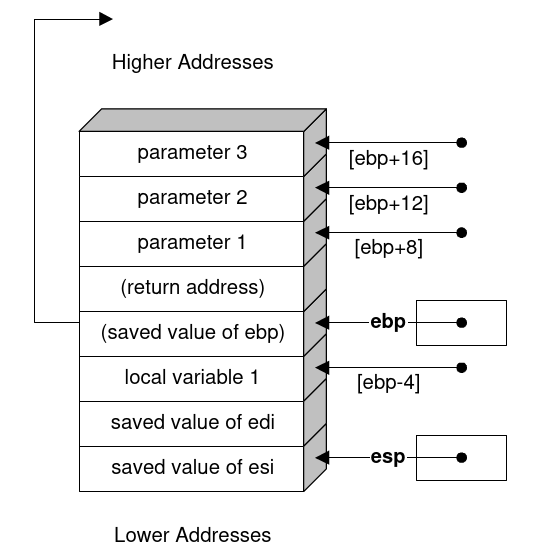
\includegraphics[width=\linewidth]{binary/archi/images/x86_stack_frame.png}
  \caption{x86 stack frame}
  \label{fig:x86_stack_frame}
\end{figure}

\subsubsection{x64 C calling Convention}
The x64 calling convention differ from the x86 in that most of the parameters
are transmitted by using registers. 
\begin{verbatim}
Register        usage
rax          Return Value
rbx          Callee Saved
rcx          4th argument
rdx          3th argument
rsi          2th argument
rdi          1th argument
rbp          Callee Saved
rsp          Stack Pointer
r8           5th Argument
r9           6th Argument
r10          Temporary
r11          Temporary
r12          Callee Saved
r13          Callee Saved
r14          Callee Saved
r15          Callee Saved
\end{verbatim}

for example the following function
\begin{verbatim}
long myfunc(long a, long b, long c, long d,
            long e, long f, long g, long h)
{
    long xx = a * b * c * d * e * f * g * h;
    long yy = a + b + c + d + e + f + g + h;
    long zz = utilfunc(xx, yy, xx % yy);
    return zz + 20;
}
\end{verbatim}

will produce the following stack frame:
 \begin{figure}
  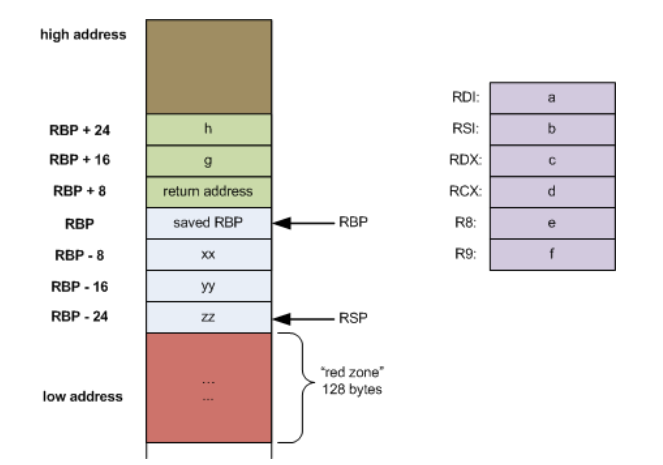
\includegraphics[width=\linewidth]{binary/archi/images/x64_stack_frame.png}
  \caption{x64 stack frame}
  \label{fig:x64_stack_frame}
\end{figure}

{\bf The red zone} The 128-byte area beyond the location pointed to by
\verb+rsp+ is considered to be reserved and shall not be modified by signal or
interrupt handlers. Therefore, functions may use this area for temporary data
that is not needed across function calls. In particular, leaf functions may use
this area for their entire stack frame, rather than adjusting the stack pointer
in the prologue and epilogue. This area is known as the red zone.


\subsection{Interrupts, Debugger traps}

 \begin{verbatim}
 int num    ; were “num” represents an interrupt handler
 \end{verbatim}

Interrupts are used to tell the CPU to halt the execution of a thread. They can
be hardware based, software based or exception based (for example unauthorized
memory access attempt). When the INT instruction is hit, the execution is moved
to an exception handler, which is defined by num. Some INT flavours do not
require a num value, INT3 for example.

When a software based breakpoint is set in an assembly level debugger the
instruction where the breakpoint is supposed to hit is exchanged to an int3
instruction, which has the hexadecimal value of \verb+0xCC+. And when the
interrupt is hit, the control of the thread is handed back to the debugger. At
the same time, the {\bf trap flag} is set. When a program is single stepped in a
debugger, the CPU is checking for the trap flag. If the trap flag is set, the
CPU will execute one instruction and give control of the thread back to the
debugger.

Again, there are other flavours of breakpoints like conditional breakpoints,
memory breakpoints and hardware breakpoints. This was just a detailed
explanation of software breakpoints to demonstrate the idea of breakpoints.

\section{links}
\href{https://www.intel.com/content/dam/www/public/us/en/documents/manuals/64-ia-32-architectures-software-developer-vol-1-manual.pdf}{Intel®
64 and IA-32 Architectures Software Developer's Manual: Basic Architecture}

\href{file:///home/benmusashi/Downloads/325383-sdm-vol-2abcd-1.pdf}{Intel 64
    and IA-32 Architectures Software Developer's Manual: Instruction Set
Reference}

\href{https://www.intel.com/content/dam/www/public/us/en/documents/manuals/64-ia-32-architectures-software-developer-system-programming-manual-325384.pdf}{Intel 64 and IA-32 Architectures Software Developer's Manual:
SystemProgramming Guide}

\href{https://faculty.nps.edu/cseagle/assembly/sys_call.html}{linux syscalls}

\href{https://www.intel.com/content/www/us/en/developer/articles/technical/intel-sdm.html}{Intel®
64 and IA-32 Architectures Software Developer Manuals}

\href{https://www.nasm.us/doc/}{NASM documentation}

\href{https://filippo.io/linux-syscall-table/}{Searchable Linux Syscall Table
for x86 and x86\_64}
